%TODO: Vikram, figure is missing
%TODO: Figure out if we can publicly share a sanitized version of the MAC instruction's timing reports
%TODO: Reconfig. in LRU? Maybe this is not even required ...
%TODO: Ensure merge strategy for bounded packet history is available in the TR
%TODO: Prove convergence of fixed point algorithm

\chapter{The Merge Procedure for Linear-in-state Functions}
\label{app:merge}

For queries that are linear in state, the state update takes the form $\mathbf{S} = A(\mathbf{p})\cdot\mathbf{S} + B(\mathbf{p})$, where $S$ is a vector of state, and $A$ and $B$ are functions of the previous $k$ packets (denoted by $\mathbf{p})$. Here $k$ is an arbitrary integer.

\section{Single packet history}

Consider the case where $k = 1$. If the state is $\mathbf{S}$ at any point in time, then after $N$ packets,
$\mathbf{S_N} = A^N\cdot \mathbf{S} + $ terms independent of $S$. Here, $A^N$ is shorthand for $A(p_N)\cdot A(p_{N-1}) \cdot \ldots \cdot A(p_1)$
Therefore to merge an evicted value $\mathbf{S_N}$ with the existing value $\mathbf{S}_{backing}$ in the backing store,
we need to replace $\mathbf{S}$ with $\mathbf{S}_{backing}$ in the expression for $\mathbf{S_N}$ by computing:
\[ \mathbf{S_N} - A^N \cdot \mathbf{S} + A^N \cdot \mathbf{S}_{backing} = \mathbf{S_N} + A^N(\mathbf{S}_{backing} - \mathbf{S}) \]
The merge procedure is straightforward: the router keeps $A^N$ as auxiliary state and passes it with $\mathbf{S_N}$ to the backing store to complete the merge.
The backing store already knows $S$, since it is the default starting value for the state, which does not change.

\section{Bounded packet history}

The required auxiliary state is more complex for larger values of $k$. If $k = 1$, $A(p)$ and $B(p)$ are known to the router for every packet. However, for larger values of $k$, the router needs access to older packet fields to compute $A(\mathbf{p})$ and $B(\mathbf{p})$. This means the values of $A$ and $B$ are themselves incorrect for the first $k-1$ packets after an eviction, an issue that must be addressed by the merge procedure.

Consider Figure~\ref{fig:bph-merge} for $k = 3$. Once the router performs an eviction at $T_1$,
the router cannot properly update the its state for the next two packets (first packets of the subsequent epoch).
It thus starts updating its state from the third packet onwards and entrusts the backing store to
fill the ``hole'' caused by missing the first two state updates.

\begin{figure}[h]
\centering
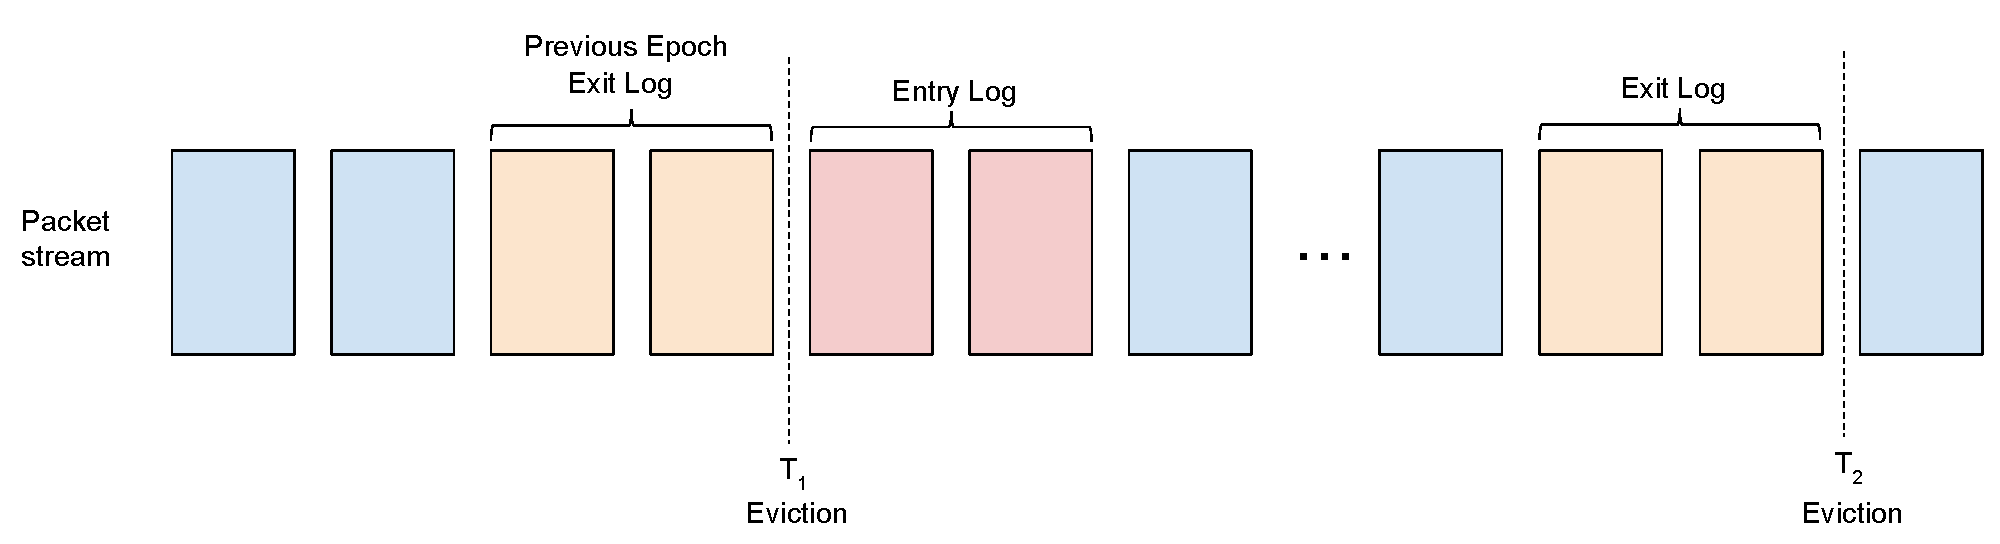
\includegraphics[width=0.7\linewidth]{pq_merge_tr_bph.pdf}
\caption{Entry and exit log for an eviction, with $k = 3$.}
\label{fig:bph-merge}
\end{figure}

To perform the merge successfully,
the backing
store needs two additions pieces of information, 
in addition to the query-specific state $A^N$ discussed in the previous section:
\begin{itemize}
\item The last $k-1$ packets from the \emph{previous epoch}, called the \emph{exit log} $R$ of the previous epoch.
\item The first $k-1$ packets from the \emph{current epoch}, called the \emph{entry log} $X$ of the current epoch. 
\end{itemize}

Upon merging, the backing store receives $S$, $R$, and $X$, and must merge them with $S_{backing}$. First, the backing store runs the actual aggregation function over $R$ starting from $S_{backing}$: $S' = g(S_{backing}, R)$. Doing this requires the backing store to use the exit log of the \emph{previous} epoch. The backing store then performs a standard merge
 $S'' = m(S', S)$ and stores $X$ for use in the \emph{next} epoch's merge.
